\chapter{串}\label{DS04}

\par\medskip\noindent\textbf{章节脉络}\par\smallskip
\begin{wideblock}\centering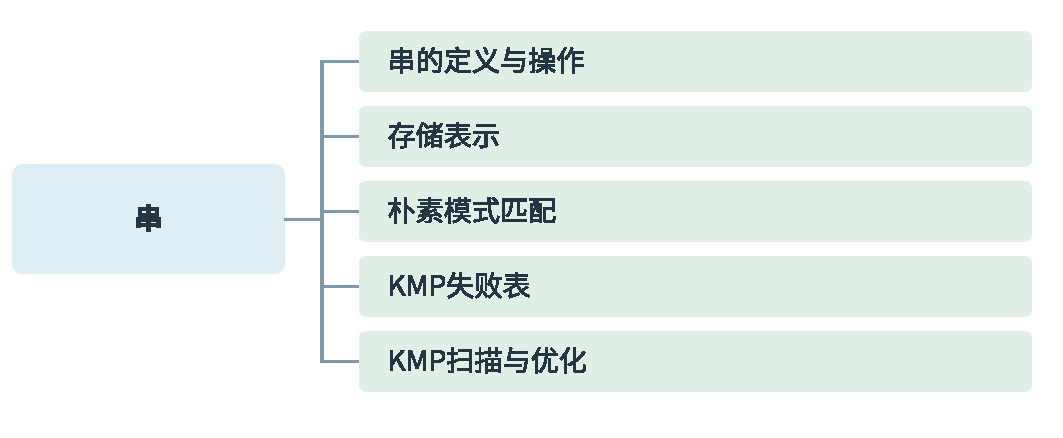
\includegraphics[width=\linewidth,height=92mm,keepaspectratio]{figures/overview.pdf}\end{wideblock}\par\medskip

串把字符序列作为一个整体处理。学习本章要同时分清三个问题：逻辑上哪些字符属于串，存储时怎样记录字符与长度，匹配时怎样利用已经比较过的信息。本章代码采用王道的顺序串表示：字符从位置1开始，\texttt{ch[\allowbreak{}0]\allowbreak{}}弃用，\texttt{length}另存串长；位置和匹配结果均按这一约定解释。

\section{字符串、子串与基本操作}\label{DS04-01}

\textbf{串}是由零个或多个字符组成的有限序列，记为\(S='a_1a_2\cdots a_n'\)；\(n\)为串长。\(n=0\)的是空串。一个或多个空格构成空格串，它含有字符，长度大于0。串中的字符可以是字母、数字、标点或其他编码字符；具体程序必须约定一个存储单元表示什么，本章算法以一个\texttt{char}为一个比较单位。

串中任意\textbf{连续}字符组成的子序列称为子串，包含该子串的串称为主串。子串在主串中的位置用其第一个字符的位置表示；同一值可能多次出现，例如\texttt{ababa}中的\texttt{aba}从位置1和3开始。模式串是要查找的串，它可能不存在于主串中；不能先把``模式串''当成已找到的子串。

两个串相等，当且仅当长度相同且每个对应字符都相同。串的大小比较采用字典序：从前向后找第一对不同字符，按约定的字符编码次序决定大小；若一方先结束且已比较部分全相同，较短串较小。例如\texttt{wang}小于\texttt{wangdao}；比较串的大小不是比较串长，也不是将整个串当成十进制数。

串属于线性结构，但串的基本操作通常以一个串或子串作为处理对象，而普通线性表常以单个数据元素为对象。赋值、比较、连接、取子串、替换与定位是不同运算，输入输出和修改对象应写清。

\begin{wideblock}

\par\medskip\noindent\begin{minipage}{\linewidth}\fontsize{9.3}{12}\selectfont\begin{tabularx}{\linewidth}{@{}YYY@{}}
\toprule\noalign{}
\begin{minipage}[b]{\linewidth}\raggedright
操作
\end{minipage} & \begin{minipage}[b]{\linewidth}\raggedright
语义与结果
\end{minipage} & \begin{minipage}[b]{\linewidth}\raggedright
需要检查的条件
\end{minipage} \\
\midrule\noalign{}


\texttt{StrAssign(\allowbreak{}T,\allowbreak{}chars)\allowbreak{}} & 将字符序列赋给T & 目标容量、字符数 \\
\texttt{StrCopy(\allowbreak{}T,\allowbreak{}S)\allowbreak{}} & 用S的值复制得到T & 独立复制还是共享存储 \\
\texttt{StrEmpty(\allowbreak{}S)\allowbreak{}}、\texttt{StrLength(\allowbreak{}S)\allowbreak{}} & 判空、取得串长 & 空串的length为0 \\
\texttt{ClearString(\allowbreak{}S)\allowbreak{}} & 使S成为空串 & 顺序串清空不必释放固定数组 \\
\texttt{DestroyString(\allowbreak{}S)\allowbreak{}} & 销毁并回收动态存储 & 堆串与定长串的资源行为不同 \\
\texttt{Concat(\allowbreak{}T,\allowbreak{}S1,\allowbreak{}S2)\allowbreak{}} & 按先后连接两串得到T & 长度之和能否容纳 \\
\texttt{SubString(\allowbreak{}Sub,\allowbreak{}S,\allowbreak{}pos,\allowbreak{}len)\allowbreak{}} & 取位置pos起、长度len的子串 & 起点、长度及末位置合法 \\
\bottomrule\end{tabularx}
\end{minipage}\par\medskip

\par\medskip\noindent\begin{minipage}{\linewidth}\fontsize{9.3}{12}\selectfont\begin{tabularx}{\linewidth}{@{}YYY@{}}
\toprule\noalign{}
\begin{minipage}[b]{\linewidth}\raggedright
操作
\end{minipage} & \begin{minipage}[b]{\linewidth}\raggedright
语义与结果
\end{minipage} & \begin{minipage}[b]{\linewidth}\raggedright
需要检查的条件
\end{minipage} \\
\midrule\noalign{}


\texttt{StrCompare(\allowbreak{}S,\allowbreak{}T)\allowbreak{}} & 返回正、零或负值表示大小关系 & 字符编码比较规则 \\
\texttt{Index(\allowbreak{}S,\allowbreak{}T)\allowbreak{}} & 返回T在S中第一次出现的位置 & 本章失败返回0 \\
\bottomrule\end{tabularx}
\end{minipage}\par\medskip

\end{wideblock}

\subsection{子串的起点和长度怎样约束}\label{DS04-bound}

设\(S\)长\(n\)，取非空子串时须满足\(1\le pos\le n\)、\(len>0\)及\(pos+len-1\le n\)。若允许空子串，可将条件扩展为\(1\le pos\le n+1\)、\(len\ge0\)及\(pos+len-1\le n\)；这时\(n+1\)只允许取长度0的串。接口采用哪种边界应明确约定。本章给出的\texttt{SubString}允许后一种情况；模式匹配的主体分析采用非空模式，空模式在调用入口约定返回位置1。

\section{顺序串、堆串与链串}\label{DS04-storage}

定长顺序存储用连续字符数组保存串，串长由独立成员表示。教材结构以\texttt{MAXLEN}指定数组单元数。结合本章位置0弃用的约定，可直接访问的字符位置是\texttt{1.\allowbreak{}.\allowbreak{}MAXLEN-1}，所以实现时维持\texttt{0<\allowbreak{}=\allowbreak{}length<\allowbreak{}MAXLEN}。若软件接口要求可保存整整MAXLEN个字符，则需要额外分配一个单元，并同步声明容量约定。

\par\medskip\noindent\begin{minipage}{\linewidth}
\begin{codeblock}[language=C++]
#define MAXLEN 255
typedef struct {
    char ch[MAXLEN];
    int length;
} SString;
\end{codeblock}
\end{minipage}\par\medskip

固定数组的容量有限。清空只需令\texttt{length=\allowbreak{}0}，旧字符即使仍留在数组中，也不再属于有效串。显式记录长度时无需用\texttt{'\textbackslash{}0'}作结束标志；若把这种串传给要求C字符串的库函数，必须额外转换表示，不能直接把\texttt{ch}作为同一种接口使用。

教材式顺序串存在不同布局：用\texttt{ch[\allowbreak{}0]\allowbreak{}}记录长度、从位置1保存字符；另设长度而从位置0保存字符；以\texttt{'\textbackslash{}0'}结束；另设长度且字符从1开始。本章统一采用最后一种。第一种还受长度单元可表示范围限制；结束符方式需要扫描才能求长，并将结束符与有效字符区分。

\textbf{堆分配存储}用指针指向动态申请的连续区，常见定义为：

\par\medskip\noindent\begin{minipage}{\linewidth}
\begin{codeblock}[language=C++]
typedef struct {
    char *ch;
    int length;
} HString;
\end{codeblock}
\end{minipage}\par\medskip

动态分配能按实际需要调整空间，代价是要管理申请、复制、释放和失败情形。赋值一个指针只复制地址，不能自动得到独立字符副本。长度改变且容量不足时，应先申请新空间，成功后搬移并释放旧区，避免申请失败后丢失原串。

\textbf{链式存储}可以每结点存一个字符，也可以每结点保存多个字符形成串块。若每字符1字节而指针4字节，单字符结点只计数据与链接时，存储密度为\(1/(1+4)=20\%\)；一个结点存4字符时可提升至\(4/(4+4)=50\%\)。实际平台指针宽度和结构体对齐还会改变字节数。块结点末尾的填充符与真实字符应靠长度或其他约定区分。

\par\medskip\noindent\begin{minipage}{\linewidth}
\centering
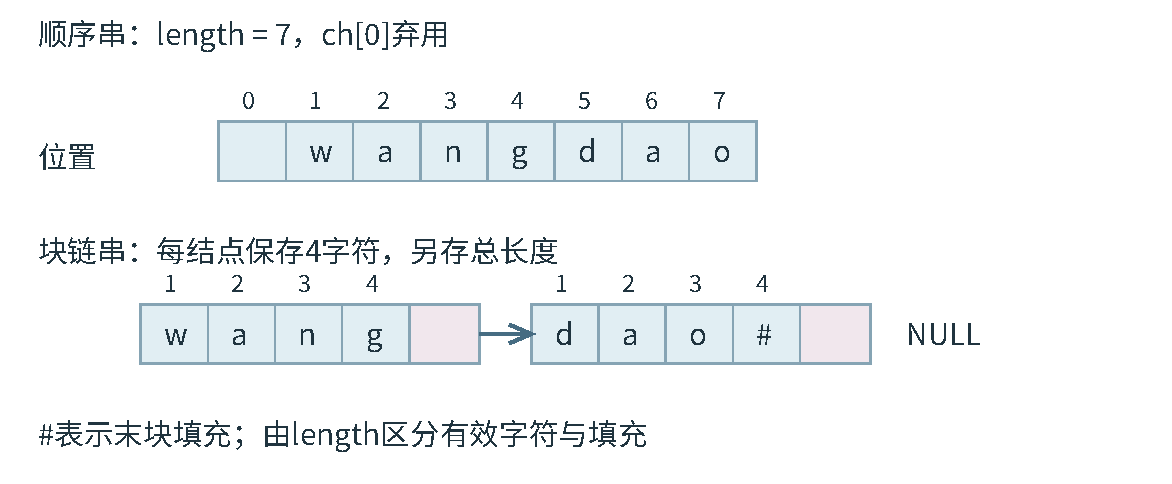
\includegraphics[width=\linewidth,height=125mm,keepaspectratio]{figures/DS04_string_layout.pdf}
\captionof{figure}{顺序串的1起始字符位置与链块串的链接关系}\label{ds04-fig-storage}
\end{minipage}\par\medskip

\section{基本操作怎样落实到代码}\label{DS04-basic-code}

\texttt{SubString}先检查范围，再从主串复制；失败时保留输出串原值。按固定数组模型，最多复制\texttt{len}个字符，时间\(O(len)\)，除返回结果外只用常数个工作变量。

\par\medskip\noindent\begin{minipage}{\linewidth}
\BlueLines{2,4,8}
\begin{codeblock}[language=C++]
bool SubString(SString &Sub, SString S, int pos, int len) {
    if (pos < 1 || pos > S.length + 1 || len < 0 ||
        len > S.length - pos + 1)
        return false;
    for (int i = pos; i < pos + len; ++i)
        Sub.ch[i - pos + 1] = S.ch[i];
    Sub.length = len;
    return true;
}
int StrCompare(SString S, SString T) {
    for (int i = 1; i <= S.length && i <= T.length; ++i)
        if (S.ch[i] != T.ch[i])
            return (unsigned char)S.ch[i] -
                   (unsigned char)T.ch[i];
    return S.length - T.length;
}
\end{codeblock}
\end{minipage}\par\medskip

比较的时间由第一次不同的位置决定，最坏\(O(\min(n,m))\)。返回值只要求正、零、负正确；不能把``返回正值''误背成``必须返回1''。转为\texttt{unsigned char}后比较，可以避免某些实现中\texttt{char}有符号导致高位编码被当作负数。

连接先检查总长，再分别复制两段。若接口允许输出与输入是同一个对象，需要按实现检查覆盖问题；下例按值接收定长顺序串，输入副本使\texttt{Concat(\allowbreak{}S,\allowbreak{}S,\allowbreak{}T)\allowbreak{}}仍能读取原来的S。

\par\medskip\noindent\begin{minipage}{\linewidth}
\BlueLines{2,8}
\begin{codeblock}[language=C++]
bool Concat(SString &T, SString S1, SString S2) {
    if (S1.length + S2.length >= MAXLEN) return false;
    for (int i = 1; i <= S1.length; ++i)
        T.ch[i] = S1.ch[i];
    for (int i = 1; i <= S2.length; ++i)
        T.ch[S1.length + i] = S2.ch[i];
    T.length = S1.length + S2.length;
    return true;
}
\end{codeblock}
\end{minipage}\par\medskip

若用字符串基本操作描述朴素定位，可以依次取长度\(m\)的子串，再用\texttt{StrCompare}比较。非空模式最多有\(n-m+1\)个候选起点；模式长于主串时没有候选。下面改用字符位置直接实现，能更清楚地看到回溯和字符比较次数。

\section{朴素匹配：失败后移到下一个起点}\label{DS04-02}

令\texttt{i}指主串当前比较字符，\texttt{j}指模式当前比较字符，二者都从1开始。相等时同时递增；不等时，已经比较的模式前缀长为\(j-1\)，本轮起点是\(i-j+1\)，下一个起点是\(i-j+2\)，因此执行\texttt{i=\allowbreak{}i-j+\allowbreak{}2;\allowbreak{} j=\allowbreak{}1;\allowbreak{}}。

\par\medskip\noindent\begin{minipage}{\linewidth}
\BlueLines{2,4,5}
\begin{codeblock}[language=C++]
int Index(SString S, SString T) {
    if (T.length == 0) return 1;
    int i = 1, j = 1;
    while (i <= S.length && j <= T.length) {
        if (S.ch[i] == T.ch[j]) {
            ++i; ++j;
        } else {
            i = i - j + 2;
            j = 1;
        }
    }
    if (j > T.length) return i - T.length;
    return 0;
}
\end{codeblock}
\end{minipage}\par\medskip

成功时，\texttt{j=\allowbreak{}m+\allowbreak{}1}，\texttt{i}已越过匹配段，起点为\(i-m\)。主串先耗尽而模式仍未完成时失败，返回0。失败值0与合法位置1区分，不应改用另一个接口的\texttt{-1}。

\subsection{例：按课件主串逐次尝试}\label{DS04-naive-example}

主串\texttt{S=\allowbreak{}abaabaabcabaabc}，模式\texttt{T=\allowbreak{}abaabc}。起点1处前5字符相同，第6字符\texttt{a}与\texttt{c}失配；起点2的\texttt{b}与模式首字符\texttt{a}失配；起点3先比较一个\texttt{a}，下一字符\texttt{a}与\texttt{b}失配；起点4的6个字符全部相等，第一次成功位置为4。

\par\medskip\noindent\begin{minipage}{\linewidth}\fontsize{9.3}{12}\selectfont\begin{tabularx}{\linewidth}{@{}YYY@{}}
\toprule\noalign{}
尝试起点 & 本轮字符比较次数 & 结果 \\
\midrule\noalign{}


1 & 6 & 第6对失配 \\
2 & 1 & 第1对失配 \\
3 & 2 & 第2对失配 \\
4 & 6 & 全部匹配 \\
\bottomrule\end{tabularx}
\end{minipage}\par\medskip

合计15次字符比较。这个总数属于这一组数据，不能当作算法的一般复杂度。

最坏情形如主串前部有大量\texttt{a}、模式为\texttt{aaaab}：每个起点都在接近末尾处失败，时间为\(O((n-m+1)m)\)，通常简记\(O(nm)\)。若首起点就完全匹配，则只比较\(m\)次；讨论最好情况时须说明是否保证成功及是否把建表等准备工作计入。

\section{KMP：利用已相等部分决定回退}\label{DS04-03}

设在位置\(i,j\)失配。此前有

\[S[i-j+1..i-1]=T[1..j-1].\]

这段主串已经被证明等于模式前缀。模式右移后仍能保留的部分，必须同时是\(T[1..j-1]\)的真后缀和模式的真前缀。设最长相等真前后缀长为\(k\)，那么前\(k\)字符无需再比较，下一次应将模式位置\(k+1\)与同一个主串字符比较。

因此，对\(j>1\)定义

\[next[j]=1+\text{串 }T[1..j-1]\text{ 的最长相等真前后缀长度},\]

并定义\(next[1]=0\)。\texttt{next[\allowbreak{}j]\allowbreak{}}保存的是\textbf{下次比较的位置}，不是直接保存前后缀长度。值0是首字符失配后的特殊状态：下一轮同时令\texttt{i}和\texttt{j}递增，主串进入下一字符，模式恢复到位置1。

\par\medskip\noindent\begin{minipage}{\linewidth}
\centering
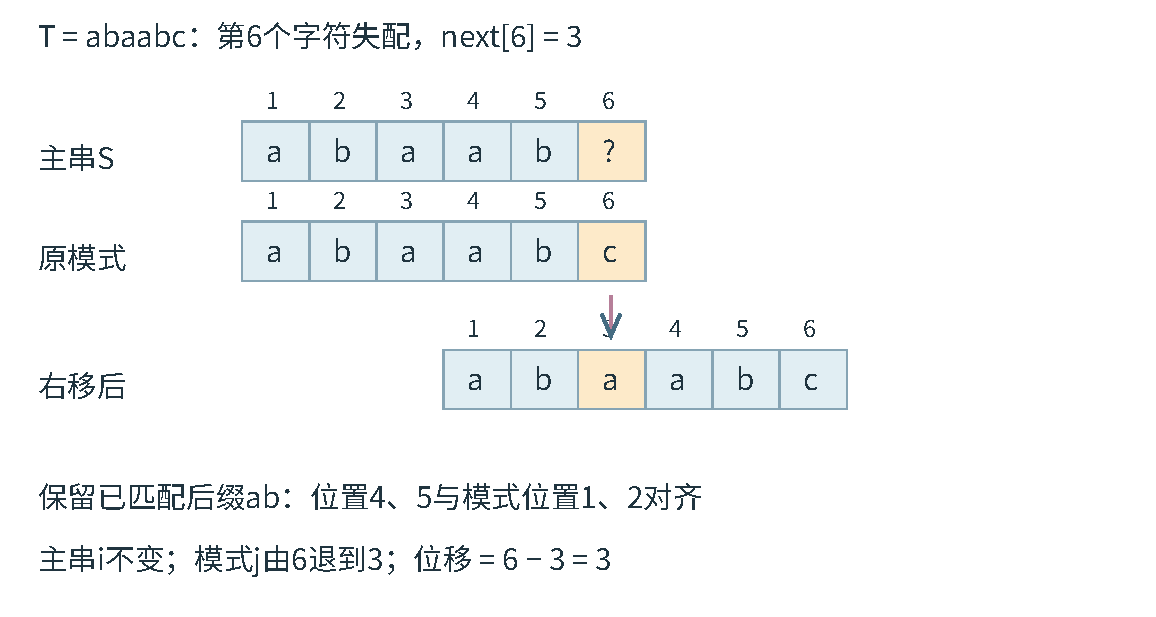
\includegraphics[width=\linewidth,height=125mm,keepaspectratio]{figures/DS04_kmp_1based.pdf}
\captionof{figure}{abaabc在第6位置失配后，已匹配段的后缀ab与模式前缀ab对齐，j由6退到3}\label{ds04-fig-kmp}
\end{minipage}\par\medskip

模式\texttt{abaabc}的普通next为：

\begin{wideblock}\par\medskip\noindent\begin{minipage}{\linewidth}\fontsize{9.3}{12}\selectfont\begin{tabularx}{\linewidth}{@{}YYYYYYY@{}}
\toprule\noalign{}
位置j & 1 & 2 & 3 & 4 & 5 & 6 \\
\midrule\noalign{}


T.ch{[}j{]} & a & b & a & a & b & c \\
j之前的串 & 空 & a & ab & aba & abaa & abaab \\
最长相等真前后缀长 & 特殊 & 0 & 0 & 1 & 1 & 2 \\
next{[}j{]} & 0 & 1 & 1 & 2 & 2 & 3 \\
\bottomrule\end{tabularx}
\end{minipage}\par\medskip\end{wideblock}

例如\(j=6\)前的串是\texttt{abaab}，最长相等真前后缀为\texttt{ab}，长2，所以\texttt{next[\allowbreak{}6]\allowbreak{}=\allowbreak{}3}。当第6字符失配时，只改变\texttt{j}到3，\texttt{i}不变；不是把模式移到主串位置3。

\par\medskip\noindent\begin{minipage}{\linewidth}
\BlueLines{2,4,5}
\begin{codeblock}[language=C++]
int Index_KMP(SString S, SString T, int next[]) {
    if (T.length == 0) return 1;
    int i = 1, j = 1;
    while (i <= S.length && j <= T.length) {
        if (j == 0 || S.ch[i] == T.ch[j]) {
            ++i;
            ++j;
        } else {
            j = next[j];
        }
    }
    if (j > T.length) return i - T.length;
    return 0;
}
\end{codeblock}
\end{minipage}\par\medskip

短路求值使\texttt{j=\allowbreak{}=\allowbreak{}0}时不访问\texttt{T.\allowbreak{}ch[\allowbreak{}0]\allowbreak{}}。模式在逻辑上右移，主串指针单调递增；同一个主串字符仍可能与多个模式位置比较，所以不能将KMP解释成``每个主串字符恰好比较一次''。

\subsection{例：同一主串上的KMP轨迹}\label{DS04-kmp-example}

仍取\texttt{S=\allowbreak{}abaabaabcabaabc}、\texttt{T=\allowbreak{}abaabc}。先比较位置\((1,1)\)至\((5,5)\)成功，在\((6,6)\)失配。由\texttt{next[\allowbreak{}6]\allowbreak{}=\allowbreak{}3}，下一次比较\((6,3)\)，主串位置6的\texttt{a}等于模式位置3的\texttt{a}；随后比较\((7,4)\)、\((8,5)\)、\((9,6)\)都成功。此时\texttt{i=\allowbreak{}10,\allowbreak{}j=\allowbreak{}7}，返回\(10-6=4\)。

\begin{wideblock}\par\medskip\noindent\begin{minipage}{\linewidth}\fontsize{9.3}{12}\selectfont\begin{tabularx}{\linewidth}{@{}YYYY@{}}
\toprule\noalign{}
阶段 & 主串位置i & 模式位置j & 操作 \\
\midrule\noalign{}


已有5字符相等 & 6 & 6 & a与c失配 \\
查next & 6 & 3 & 主串位置不变 \\
继续比较 & 6、7、8、9 & 3、4、5、6 & 连续4对相等 \\
完成 & 10 & 7 & 返回位置4 \\
\bottomrule\end{tabularx}
\end{minipage}\par\medskip\end{wideblock}

本例普通KMP共比较10次字符，少于朴素的15次；判断\texttt{j=\allowbreak{}=\allowbreak{}0}不算一对字符比较。另一课件主串\texttt{abaacaabcabaabc}会产生连续回退：在\(i=5,j=5\)失配后\(j=2\)，仍失配再退\(j=1\)，再失配退\(j=0\)；此后推进主串到\(i=6,j=1\)。连续回退只查表，不让主串后退。

\section{怎样在线性时间内求next}\label{DS04-next}

求表也可看成模式串与自身前缀的匹配。设正在求\texttt{next[\allowbreak{}i+\allowbreak{}1]\allowbreak{}}，已知\texttt{next[\allowbreak{}i]\allowbreak{}=\allowbreak{}j}。若\texttt{j=\allowbreak{}=\allowbreak{}0}或\texttt{T.\allowbreak{}ch[\allowbreak{}i]\allowbreak{}=\allowbreak{}=\allowbreak{}T.\allowbreak{}ch[\allowbreak{}j]\allowbreak{}}，当前相等前后缀可扩展一字符，故\texttt{next[\allowbreak{}i+\allowbreak{}1]\allowbreak{}=\allowbreak{}j+\allowbreak{}1}；否则先尝试更短的候选边界，令\texttt{j=\allowbreak{}next[\allowbreak{}j]\allowbreak{}}。

\par\medskip\noindent\begin{minipage}{\linewidth}
\BlueLines{2,5,6}
\begin{codeblock}[language=C++]
void get_next(SString T, int next[]) {
    if (T.length == 0) return;
    int i = 1, j = 0;
    next[1] = 0;
    while (i < T.length) {
        if (j == 0 || T.ch[i] == T.ch[j]) {
            ++i; ++j;
            next[i] = j;
        } else {
            j = next[j];
        }
    }
}
\end{codeblock}
\end{minipage}\par\medskip

这里的\texttt{i}是模式串内部的工作位置，与匹配函数的主串工作位置作用不同。\texttt{while(\allowbreak{}i<\allowbreak{}T.\allowbreak{}length)\allowbreak{}}保证递增后最多写到\texttt{next[\allowbreak{}T.\allowbreak{}length]\allowbreak{}}。若使用另一种定义而把\texttt{next}记成前缀函数，表值和匹配代码就必须一起换；本章始终使用教材的下一比较位置定义。

\subsection{三组课件手算练习}\label{DS04-next-practice}

\par\medskip\noindent\begin{minipage}{\linewidth}\fontsize{9.3}{12}\selectfont\begin{tabularx}{\linewidth}{@{}YYY@{}}
\toprule\noalign{}
模式串 & 位置 & 普通next \\
\midrule\noalign{}


google & 1、2、3、4、5、6 & 0、1、1、1、2、1 \\
ababaa & 1、2、3、4、5、6 & 0、1、1、2、3、4 \\
aaaab & 1、2、3、4、5 & 0、1、2、3、4 \\
\bottomrule\end{tabularx}
\end{minipage}\par\medskip

\texttt{google}在位置5前的\texttt{goog}有长度1的相等真前后缀\texttt{g}，所以\texttt{next[\allowbreak{}5]\allowbreak{}=\allowbreak{}2}；位置6前的\texttt{googl}没有非空相等真前后缀，因此\texttt{next[\allowbreak{}6]\allowbreak{}=\allowbreak{}1}。\texttt{ababaa}在位置6前的\texttt{ababa}有最长边界\texttt{aba}，所以\texttt{next[\allowbreak{}6]\allowbreak{}=\allowbreak{}4}。\texttt{aaaab}每个待考察前缀都是一串\texttt{a}，其最长真边界只比它本身短1。

课件主串\texttt{googlogoogoogle}、模式\texttt{google}的匹配过程会反复利用这些边界，第一次成功位置为10。手算时先列主串和模式的位置行，再记录每一次失配后的\texttt{j}，比仅画模式移动的外形更容易核对。

\section{nextval怎样跳过必然失败的比较}\label{DS04-nextval}

若当前\texttt{S.\allowbreak{}ch[\allowbreak{}i]\allowbreak{}}与\texttt{T.\allowbreak{}ch[\allowbreak{}j]\allowbreak{}}已失配，而\texttt{T.\allowbreak{}ch[\allowbreak{}next[\allowbreak{}j]\allowbreak{}]\allowbreak{}=\allowbreak{}=\allowbreak{}T.\allowbreak{}ch[\allowbreak{}j]\allowbreak{}}，同一个主串字符与回退位置的字符也一定失配。可以继续沿失败链接，直接寻找字符不同的候选位置；把最终位置记为\texttt{nextval[\allowbreak{}j]\allowbreak{}}。

由普通next求优化表时，先令\(nextval[1]=0\)。为简化公式，记\(T[j]=T.ch[j]\)，对\(j\ge2\)有：

\[nextval[j]=\begin{cases}
next[j],&T[j]\ne T[next[j]],\\
nextval[next[j]],&T[j]=T[next[j]].
\end{cases}\]

对\(j\ge2\)，普通\texttt{next[\allowbreak{}j]\allowbreak{}}至少为1，所以该式不访问\texttt{T.\allowbreak{}ch[\allowbreak{}0]\allowbreak{}}。\texttt{nextval}使用已确认的失配信息，省去必定失败的比较，不改变匹配结果。

\par\medskip\noindent\begin{minipage}{\linewidth}\fontsize{9.3}{12}\selectfont\begin{tabularx}{\linewidth}{@{}YYY@{}}
\toprule\noalign{}
模式串 & 普通next & 优化nextval \\
\midrule\noalign{}


abaabc & 0、1、1、2、2、3 & 0、1、0、2、1、3 \\
ababaa & 0、1、1、2、3、4 & 0、1、0、1、0、4 \\
aaaab & 0、1、2、3、4 & 0、0、0、0、4 \\
\bottomrule\end{tabularx}
\end{minipage}\par\medskip

例如\texttt{abaabc}的\(j=3\)字符为\texttt{a}，而\texttt{next[\allowbreak{}3]\allowbreak{}=\allowbreak{}1}也指向\texttt{a}，故\texttt{nextval[\allowbreak{}3]\allowbreak{}=\allowbreak{}nextval[\allowbreak{}1]\allowbreak{}=\allowbreak{}0}；\(j=5\)是\texttt{b}，普通回退到2仍为\texttt{b}，故\texttt{nextval[\allowbreak{}5]\allowbreak{}=\allowbreak{}nextval[\allowbreak{}2]\allowbreak{}=\allowbreak{}1}。

\par\medskip\noindent\begin{minipage}{\linewidth}
\BlueLines{2,5,6}
\begin{codeblock}[language=C++]
void get_nextval(SString T, int nextval[]) {
    if (T.length == 0) return;
    int i = 1, j = 0;
    nextval[1] = 0;
    while (i < T.length) {
        if (j == 0 || T.ch[i] == T.ch[j]) {
            ++i; ++j;
            if (T.ch[i] != T.ch[j])
                nextval[i] = j;
            else
                nextval[i] = nextval[j];
        } else {
            j = nextval[j];
        }
    }
}
\end{codeblock}
\end{minipage}\par\medskip

将\texttt{nextval}作为\texttt{Index\_KMP}的第三个实参即可使用优化表，匹配循环不变。普通next与优化nextval的具体比较次数可以不同，算题前先确认题目采用哪一张表。

\subsection{例：重复字符使优化效果更明显}\label{DS04-opt-example}

主串\texttt{aaacaaaabdaaaab}，模式\texttt{aaaab}。普通next在主串位置4的\texttt{c}处，会依次与模式位置4、3、2、1的\texttt{a}失配；优化表在位置4第一次失配后直接退到0，跳过另外三次注定失败的比较。之后从主串位置5开始匹配，位置5至9恰为\texttt{aaaab}，故返回5。普通next共比较12次，nextval共比较9次。

\section{正确性、代价和容易混淆的边界}\label{DS04-analysis}

KMP正确性的关键是：每一次跳过的对齐位置都被已经相等的前缀与后缀关系排除。模式右移后还能与旧匹配段重合的部分必须是一个边界；先尝试最长边界，失败后沿next链尝试更短边界，因此不遗漏仍可能成功的起点。

建表过程中，\texttt{i}最多递增\(m-1\)次；回退使\texttt{j}减小，而\texttt{j}的总增量受\texttt{i}的推进限制，故总工作\(O(m)\)。匹配中，主串指针\texttt{i}最多递增\(n\)次，每次成功比较使\texttt{j}增加，每次失败回退使\texttt{j}减少；累积回退量仍受此前的推进约束，因此匹配扫描为\(O(n)\)。总时间\(O(n+m)\)，next数组辅助空间\(O(m)\)。只有``已给next''的匹配阶段才可单独记为\(O(n)\)。

\begin{wideblock}

\par\medskip\noindent\begin{minipage}{\linewidth}\fontsize{9.3}{12}\selectfont\begin{tabularx}{\linewidth}{@{}YYY@{}}
\toprule\noalign{}
\begin{minipage}[b]{\linewidth}\raggedright
问题
\end{minipage} & \begin{minipage}[b]{\linewidth}\raggedright
本章约定或结论
\end{minipage} & \begin{minipage}[b]{\linewidth}\raggedright
易混点
\end{minipage} \\
\midrule\noalign{}


字符起始位置 & 1 & 与C数组常见0起始分别说明 \\
匹配失败 & 返回0 & 0不是合法非空匹配起点 \\
\texttt{next[\allowbreak{}j]\allowbreak{}} & 下一次比较的模式位置 & 等于边界长度加1，而非直接等于边界长度 \\
\texttt{j=\allowbreak{}=\allowbreak{}0} & 下轮推进主串并恢复j=1 & 不是读取第0个字符 \\
字符比较次数 & 实际执行的字符相等判断 & \texttt{j=\allowbreak{}=\allowbreak{}0}、循环条件不是字符对比较 \\
匹配成功后继续查找 & 取决于是否查全部、是否允许重叠 & 只找首次出现的接口可立即返回 \\
\bottomrule\end{tabularx}
\end{minipage}\par\medskip

\end{wideblock}

固定数组按值传参会复制整个结构体；教材复杂度通常关注字符扫描和串长变化，容量视作预设上限。若要在可增长规模的软件实现中精确计算拷贝成本，应把接口实现成本一并计入。本章算法推导仍采用教材的字符比较模型。

\section{主动回忆与自查}\label{DS04-check}

以下为自拟检查题，串的位置和next均采用本章约定。

\begin{enumerate}
\def\labelenumi{\arabic{enumi}.}
\tightlist
\item
  空串和只含三个空格的串长度分别是多少？\texttt{abc}是不是\texttt{ac}的主串？
\item
  长度7的串取\texttt{pos=\allowbreak{}6,\allowbreak{}len=\allowbreak{}2}是否合法？\texttt{pos=\allowbreak{}8,\allowbreak{}len=\allowbreak{}0}呢？
\item
  字符位置为1起始时，朴素匹配在\((i,j)=(8,4)\)失配，下一个起点和新的指针分别是什么？
\item
  写出\texttt{abaabc}、\texttt{ababaa}、\texttt{aaaab}的next与nextval，解释\texttt{next[\allowbreak{}6]\allowbreak{}=\allowbreak{}3}中3的含义。
\item
  KMP在同一个主串字符上连续失配，会改变哪个指针？何时才推进主串？
\item
  对\texttt{S=\allowbreak{}abaabaabcabaabc,\allowbreak{}T=\allowbreak{}abaabc}，朴素与普通KMP第一次成功位置及字符比较次数分别是多少？
\item
  对\texttt{S=\allowbreak{}aaacaaaabdaaaab,\allowbreak{}T=\allowbreak{}aaaab}，普通next和优化nextval各比较多少次？
\item
  空模式由接口约定返回1时，是否需要访问next{[}1{]}？若模式长于主串，返回什么？
\item
  只给匹配扫描的\(O(n)\)，为何不足以说明整个KMP的准备与扫描代价？
\end{enumerate}

\subsection{核对答案}\label{DS04-answers}

\begin{enumerate}
\def\labelenumi{\arabic{enumi}.}
\tightlist
\item
  分别为0和3；\texttt{ac}不是\texttt{abc}中的连续子串。2. 均合法；第二种取得串尾后的空串。3. 本轮起点为5，下一个为6，执行\texttt{i=\allowbreak{}6,\allowbreak{}j=\allowbreak{}1}。4. next和nextval分别见上表；3表示下一比较位置，保留的是长2的边界\texttt{ab}。5. 令\texttt{j=\allowbreak{}next[\allowbreak{}j]\allowbreak{}}或\texttt{j=\allowbreak{}nextval[\allowbreak{}j]\allowbreak{}}；字符相等或j退到0后推进主串。6. 都返回4；朴素15次，普通KMP10次。7. 分别12次、9次。8. 不需要建表或访问表；非空模式长于主串时返回0。9. 还要把\(O(m)\)建表时间和\(O(m)\)表空间计入，总时间\(O(n+m)\)。
\end{enumerate}
